% Document
\begin{multicols}{2}

\section{Implementation}\label{sec:Implementation}

\subsection{Wolf Sheep Predation model as simuland}\label{subsec:simuland-wsp}
    The simuland was studied through observation of the simuland's code,
    which was written in the NetLogo programming language.
    Unlike Python, NetLogo is procedural, so we reevaluated the logic from an
    object-oriented perspective.
    We scrutinized all the methods and data in the simuland and found that it
    could be classified based on the agent it was associated with:
    (a wolf, a sheep, or a patch of grass or dirt).
    We then documented the simuland's logic, organizing information by its
    associated agent.

\subsection{Python and Mesa}\label{subsec:python-and-mesa}
    Our team decided to use the Python programming language to implement our model
    of the NetLogo simulation for three main reasons:
    1) all team members were familiar with Python already;
    2) Python has powerful third-party libraries such as numpy, pandas, and arcade;
    and 3) it is an object-oriented language.

    Soon after deciding upon a programming language for the model,
    we discovered the Mesa framework, of which had many desirable features
    which replicate our simuland.
    Mesa defines base classes for the model and agent,
    and has many built-in components which make agent-based modeling easier [Kazil, 2020].
    One component which is crucial in our model is the agent scheduler;
    our model uses the RandomActivation scheduler, which is roughly equivalent
    to NetLogo's ask procedure which reads in each agent in an
    agentset in a random order. [Wilensky 1997]
    Like the NetLogo implementation, one scheduler is instantiated for each of the
    three agent types (wolves, sheep, and patches).
    Another critical component is the grid, which is needed to represent the positions
    of each agent over the course of the simulation;
    for this, our model uses a single MultiGrid object, which has useful methods
    for placing, moving, and removing agents.
    ContinuousSpace is another spatial component which was initially considered,
    as wolves and sheep actually move with floating-point coordinates;
    however, complications arose since sheep and wolves are supposed to eat whatever
    resources are available on their current patch (which are represented by discrete
    locations) -- so the former spatial component was chosen instead.

    One of the most important aspects of Mesa lies in its powerful built-in
    visualization tools, which allow for real-time visualization and data analysis
    of the model using a browser-based interface. [Project Mesa Team 2016]
    This was particularly useful when debugging any errors which existed in the
    implementation.
    Two visualization modules used within our model are the CanvasGrid to visualize the
    individual agents, as well as the ChartModule to visualize their populations over
    time as a line graph.
    Mesa also includes UI features such as sliders to allow for easy parameterization
    of the model's initial state.

%\begin{figure}[H]
%   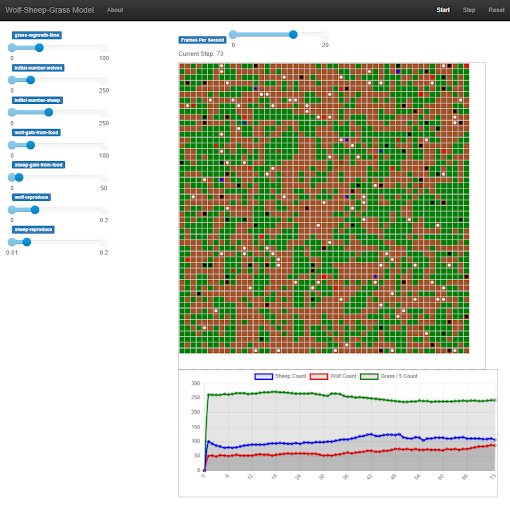
\includegraphics[width=\linewidth]{./figures/mesa_wsg}
%   \caption{\textit{
%       Real-time visualization of Wolf Sheep Predation model using Mesa framework.}}
%   \label{fig:Mesa WSP}
%\end{figure}

\subsection{Reimplemented Model}\label{subsec:reimplemented-model}
    Terrain is modeled as a 51 by 51 grid of 15 square pixels.
    A pixel is green when grass exists and brown when sheep have eaten the grass.
    The wolves and sheep move about on the grid exploring the environment to find
    food and maintain their health.

    Figure~\ref{fig:Mesa WSP} depicts a real-time visualization of the reimplemented model.
    White circles represent sheep, while black squares represent wolves.
    Green and brown squares represent grass and dirt patches, respectively.
    Additionally, newly reproduced wolves and sheep are colored blue,
    while wolves and sheep that are on the verge of starvation are colored red.
    The graph located beneath the grid shows the population of wolves, sheep,
    and grass patches over each step or tick.
    The "Frames Per Second" slider at the top adjusts the tick rate of the model,
    while the sliders on the left allow for customization of initial parameters.
    Finally, the buttons at top right allow for the user to start and stop the model,
    proceed to the next step, and reset the model.

    Code Excerpt 1 shows the Python implementation of the constructor for the
    Wolf-Sheep-Grass model.
    Line 1 gives the class definition of WolfSheepGrass,
    which inherits from the base class as defined in mesa.Model.
    Line 3 defines its constructor and its parameters.
    width and height define the dimensions of the grid-based world.
    grass\_regrowth\_rate is an integer between 0 and 100 (inclusive) which
    determines when dirt grows to grass.
    initial\_wolves and initial\_sheep are integers between 0 and 250 (inclusive)
    to spawn the initial number of animals in the simulation.
    wolf\_food\_gain and sheep\_food\_gain are integers which determine
    how much energy the animal gains from eating food;
    possible values range from 0--100 for the former and 0--50 for the latter.
    wolf\_reproduce and sheep\_reproduce determine the percent chance of the
    respective animal spawning a child of its type, ranging from 0\% to 20\%.
    Finally, max\_sheep defines the maximum number of sheep allowed;
    if no wolves are alive, and the count of sheep exceeds this number,
    the simulation ends.

    Line 5 calls the constructor of the Model class
    (which WolfSheepGrass derives from).
    Line 7--8 saves the width, height, and maximum number of sheep allowed
    in the simulation for later use.
    Line 10 and lines 12--14 instantiate the MultiGrid and RandomActivation objects
    as discussed earlier, respectively.

    Lines 16--23 initialize sheep\_schedule and the shared grid with the initial
    number of Sheep objects at random xy-coordinates;
    lines 25--32 follow similarly, initializing Wolf objects to the wolf\_schedule
    and adding them to the same grid.
    The Wolf and Sheep classes only differ in their eating behaviors,
    so in the implementation, they derive from an Animal class
    (which itself derives from the mesa.Agent class).
    Each animal is initialized with a random direction between 0 and 360 degrees,
    as well as a random amount of energy between 0 and 2 times that animal's food gain.

    Finally, lines 34--40 initialize the environment by creating Patch objects
    to patch\_schedule and to the shared grid.
    Each Patch object has a 50\% probability to be generated as grass upon
    instantiation (likewise, it has an equal probability to be generated as dirt).

    Our model comes close to replicating the NetLogo model,
    but it is different in one notable way: NetLogo uses turtles to move the wolves
    and sheep around the environment.
    It does so by rotating the turtle between 0 and 50 degrees once towards the
    right, then again towards the left, then finally moving the turtle
    forward by one step.
    Our model does not utilize turtles;
    while a turtle library exists for Python,
    it was preferable instead to use trigonometric functions for calculating
    movement by assigning a direction and xy-coordinates to wolves and sheep.
    However, this ultimately should achieve the same result with regard to an
    agent's movement.

\end{multicols}
\begin{lstlisting}[
    language=Python,
    caption={\textit{Python implementation of the Wolf Sheep Predation model's constructor.
            (The line numbers are not part of the Python code;
            they are included for ease of reference.)}},
    label={lst:code},
    breaklines=true]
from WolfSheepGrass.wsg_agent import *  # Import the agents used in the model.
from mesa import Model  # Import the Model base class.
from mesa.time import RandomActivation  # Import the scheduler for each agent.
from mesa.space import MultiGrid  # Import the grid to position and move agents.

class WolfSheepGrass(Model):
  def __init__(self, width: int, height: int,
    grass_regrowth_rate: int, initial_wolves: int, initial_sheep: int,
    wolf_food_gain: int, sheep_food_gain: int,
    wolf_reproduction_rate: float, sheep_reproduction_rate: float,
    max_sheep: int) -> None:

    super().__init__()  # Initialize the Model base class.
    self.width, self.height = width, height  # Define grid dimensions.
    self.max_sheep = max_sheep  # Don't let the number of sheep grow too large.
    self.grid = MultiGrid(width, height, True)  # Define discrete, toroidal grid.

    # Instantiate schedulers.
    self.sheep_schedule = RandomActivation(self)
    self.wolf_schedule = RandomActivation(self)
    self.patch_schedule = RandomActivation(self)

    # Add initial sheep.
    for _ in range(initial_sheep):
      x_pos, y_pos = self.random.uniform(0, width), self.random.uniform(0, height)
      sheep = Sheep(self, x_pos, y_pos, sheep_food_gain, sheep_reproduction_rate)
      self.sheep_schedule.add(sheep)
      self.grid.place_agent(sheep, (x_pos, y_pos))

    # Add initial wolves.
    for _ in range(initial_wolves):
      x_pos, y_pos = self.random.uniform(0, width), self.random.uniform(0, height)
      wolf = Wolf(self, x_pos, y_pos, wolf_food_gain, wolf_reproduction_rate)
      self.wolf_schedule.add(wolf)
      self.grid.place_agent(wolf, (x_pos, y_pos))

    # Initialize the environment.
    for x in range(width):
      for y in range(height):
        patch = Patch(self, grass_regrowth_rate, (x, y))
        self.patch_schedule.add(patch)
        self.grid.place_agent(patch, (x, y))
\end{lstlisting}

\begin{multicols}{2}

\subsection{Visualization and Validation}\label{subsec:visualization-and-validation}
    As a means of establishing model validity, the two models' animated
    visualizations were compared.
    For this purpose, the Wolf Sheep Predation model developed for this
    project was extended to a graphical representation of the simulation.
    The graphical representation included an animated representation of the
    Wolf Sheep Predation simulation, and a graph depicting the populations
    of wolves, sheep, and grass over time.
    Figure 4 shows the animation output simulation with the NetLogo runtime model.
    Casual inspection suggests that the graphical representations are comparable.
    The observed run-time behavior of the simulations is also similar.

%\begin{figure}[H]
%    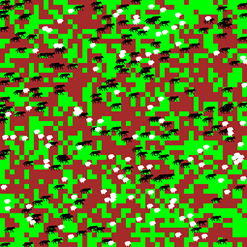
\includegraphics[width=\linewidth]{./figures/arcade_wsg}
%    \caption{\textit{
%        Model of a predator-prey relationship demonstrating the oscillating behavior.
%        As the prey species (blue) increases, it triggers an increase in the
%        predator (black) species.
%        This will cause the prey to die off, followed by the predator.
%        This cycle repeats indefinitely in the continuous case.}}
%    \label{fig:arcade_wsg}
%\end{figure}

    Figure 5 shows population graphs generated the NetLogo model and Python/Mesa model.
    Although the axis scales of the graphs differ, the overall behavior of the simulations
    is very similar in terms of the oscillating behavior of the populations.
    In both models, an increase in the sheep population is followed by a decline
    in the grass and an increase in the wolf population.
    The increased wolf population then causes a decrease in the sheep population,
    allowing the grass population to recover, and the cycle repeats.

    As mentioned, the purpose of this project was to gain experience with
    agent-based modeling.
    A different project emphasizing verification and validation methods came later
    in the course.
    Had verification and validation been a focus this project, more rigorous methods,
    such as those described in [Petty, 2010], would have been used.

%\begin{figure}[H]
%    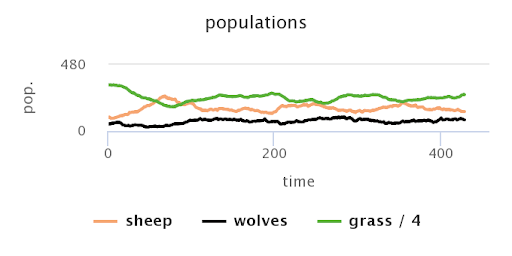
\includegraphics[width=\linewidth]{./figures/netlogo_population}
%    \caption{\textit{
%        Model of a predator-prey relationship demonstrating the oscillating behavior.
%        As the prey species (blue) increases, it triggers an increase in the
%        predator (black) species.
%        This will cause the prey to die off, followed by the predator.
%        This cycle repeats indefinitely in the continuous case.}}
%    \label{fig:netlogo_population}
%\end{figure}

%\begin{figure}[H]
%    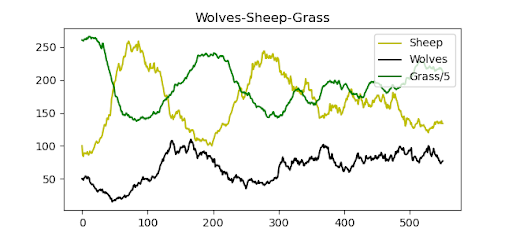
\includegraphics[width=\linewidth]{./figures/mesa_population}
%    \caption{\textit{
%        Model of a predator-prey relationship demonstrating the oscillating behavior.
%        As the prey species (blue) increases, it triggers an increase in the
%        predator (black) species.
%        This will cause the prey to die off, followed by the predator.
%        This cycle repeats indefinitely in the continuous case.}}
%    \label{fig:mesa_population}
%\end{figure}

